\documentclass[12pt]{article}
\usepackage[utf8]{inputenc}
\usepackage[T1]{fontenc}
\usepackage{geometry}
\usepackage{hyperref}
\usepackage{graphicx}
\usepackage{booktabs}
\usepackage{enumitem}
\usepackage{xcolor}

\geometry{a4paper, margin=1in}
\hypersetup{
    colorlinks=true,
    linkcolor=blue,
    urlcolor=blue,
    pdftitle={CI Workflow YAML Bug Report}
}

\title{CI Workflow YAML Bug Report Outline}
\author{Mark Samuel (202201857)}
\date{\today}

\begin{document}

\maketitle


\section{Repository Evidence}
\subsection{Public GitHub Repository Link}
\textbf{Repository URL:} \url{https://github.com/marksamfd/MLopsAssignment}

\subsection{Successful Actions Run Screenshot}
Insert a screenshot of the green workflow run from the GitHub ``Actions'' tab.
\begin{figure}[h!]
    \centering
    % Replace with your real screenshot path/file name.
    \IfFileExists{images/actions-green-run.png}{%
        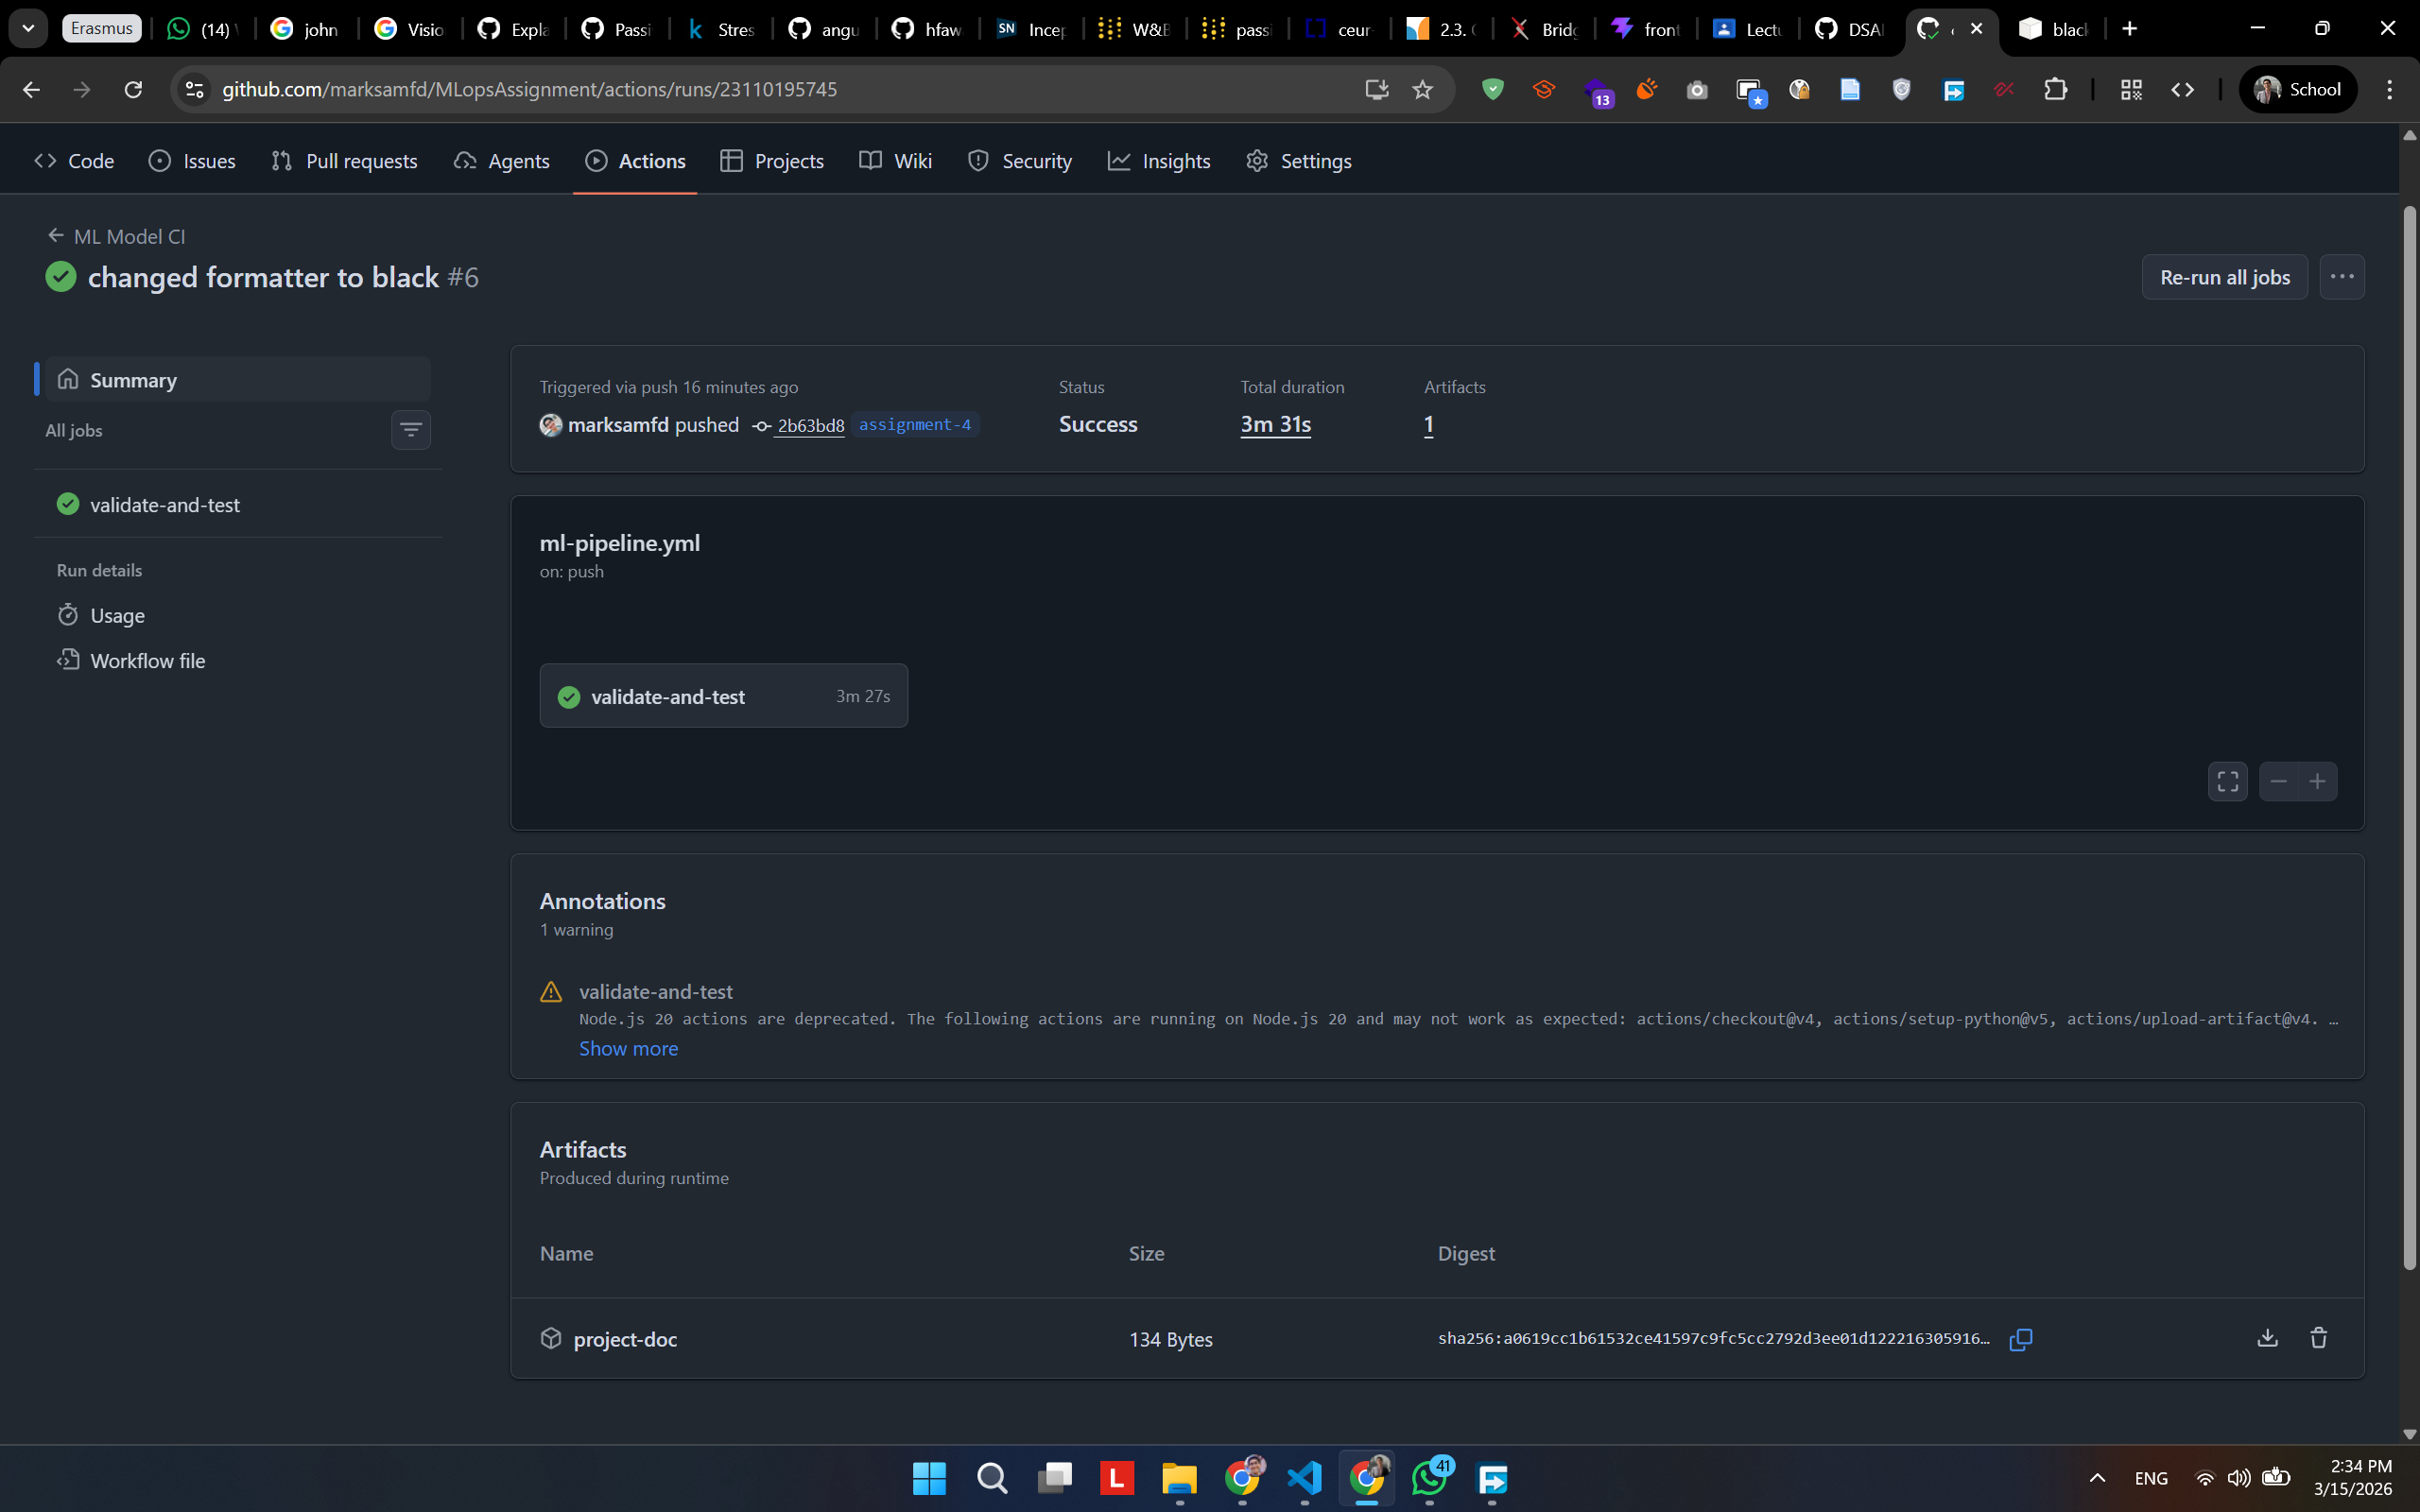
\includegraphics[width=0.95\textwidth]{images/actions-green-run.png}%
    }{%
        \fbox{\parbox[c][5cm][c]{0.9\textwidth}{\centering Screenshot placeholder:\\ images/actions-green-run.png}}%
    }
    \caption{Successful GitHub Actions run (green status).}
    \label{fig:actions-green-run}
\end{figure}

\newpage

\section{Bug Inventory in YAML File}
For each bug, use one subsection with the template below.

\subsection{Bug 1: File indentation}
\begin{itemize}[leftmargin=*]
    \item \textbf{Observed Problem:} all of file's indentation was not correct
\end{itemize}

\subsection{Bug 2: Repository Checkout was missing}
\begin{itemize}[leftmargin=*]
    \item \textbf{Observed Problem:} the CI job couldn't find requirements.txt
    \item \textbf{Fix Applied:} added action/checkout
\end{itemize}

\subsection{Bug 3: Linter Check job}
\begin{itemize}[leftmargin=*]
    \item \textbf{Observed Problem:} it had no script or workflow to run
    \item \textbf{Fix Applied:} added script to install black and check for linting errors
\end{itemize}



\section{Final Validation}
\begin{itemize}[leftmargin=*]
    \item \#6 run as successful workflow.
    \item All jobs successfully
    \item Readme file is uploaded to artifacts
\end{itemize}

\end{document}
